% Provenance (never printed): cycle 3 "La planete Terre" and geography
% (weather and climate; reading a climate chart; the great climate zones of
% the world, hot, temperate and cold); see sources/book1/PROVENANCE.md.
% Book 1, grade 5, chapter 2.
\chapter{मौसम और जलवायु}\label{ch:g5:weather-and-climate}

जनवरी के दूसरे हफ़्ते में स्कूल में दो पोस्टकार्ड आते हैं। पहला, लीना की चचेरी
बहन का, ताड़ के पेड़ों के नीचे धूप वाले \omterm{def:g2:water-on-earth:ocean}{समुद्र} \omterm{def:g1:landscapes-around-us:water}{तट} पर \omterm{def:g3:stones-pebbles-sand:sand}{रेत} का महल बनाते बच्चों को
दिखाता है। दूसरा, टॉम की दादी का, \omterm{def:g4:clouds-rain-snow:precipitation}{हिम} से ढके एक बग़ीचे में हिम-पुतला बनाते बच्चों
को दिखाता है। ``एक ही हफ़्ते में गर्मी और सर्दी दोनों कैसे हो सकती हैं?'' टॉम
पूछता है।

दोनों जगहों के बीच इतना अलग किसी एक दिन का \omterm{def:g1:watching-the-weather:weather}{मौसम} नहीं है। अलग है वह \omterm{def:g1:watching-the-weather:weather}{मौसम} जो उनके
यहाँ साल-दर-साल रहता है: उनकी \omterm{def:g5:weather-and-climate:climate}{जलवायु}।

\begin{omfigure}
\begin{minipage}[b]{0.48\linewidth}\centering

\includegraphics[width=\linewidth]{images/book1/ai/g5-beach-postcard.jpg}
\end{minipage}\hfill
\begin{minipage}[b]{0.48\linewidth}\centering

\includegraphics[width=\linewidth]{images/book1/ai/g5-snowman-postcard.jpg}
\end{minipage}

{\small जनवरी के एक ही हफ़्ते के दो पोस्टकार्ड: धूप वाला \omterm{def:g2:water-on-earth:ocean}{समुद्र} \omterm{def:g1:landscapes-around-us:water}{तट} और \omterm{def:g4:clouds-rain-snow:precipitation}{हिम} से ढका
बग़ीचा।}
\end{omfigure}

\begin{recall}
\omterm{def:g1:watching-the-weather:weather}{मौसम} किसी दी हुई जगह और समय पर हवा की दशा है: धूप, \omterm{def:g4:clouds-rain-snow:cloud}{बादल}, \omterm{def:g4:clouds-rain-snow:precipitation}{बारिश}, \omterm{def:g4:clouds-rain-snow:precipitation}{हिम}, हवा
(\cref{ch:g1:watching-the-weather})। तापमापी हवा का तापमान डिग्री सेल्सियस में
नापता है; \omterm{def:g4:clouds-rain-snow:rain-gauge}{वर्षामापी} \omterm{def:g4:clouds-rain-snow:precipitation}{बारिश} को मिलीमीटर में नापता है
(\cref{ch:g4:clouds-rain-snow})। \omterm{def:g3:continents-and-oceans:equator}{भूमध्य रेखा} \omterm{def:g3:continents-and-oceans:globe}{ग्लोब} के बीचोंबीच चारों ओर जाती है,
\omterm{def:g3:continents-and-oceans:poles}{उत्तरी ध्रुव} और \omterm{def:g3:continents-and-oceans:poles}{दक्षिणी ध्रुव} के ठीक आधे रास्ते पर
(\cref{ch:g3:continents-and-oceans})। भौतिकी की पुस्तकों ने दिखाया कि पृथ्वी एक
साल में सूर्य के चारों ओर घूमती है, और उसकी ऋतुएँ उसके अक्ष के झुकाव से आती हैं:
गर्मी में सूर्य आसमान में ज़्यादा ऊँचा चढ़ता है और दिन
लंबे होते हैं।
\end{recall}

\section{मौसम आज की बात है, जलवायु आम बात}

\omterm{def:g1:watching-the-weather:weather}{मौसम} दिन-ब-दिन, और घंटे-दर-घंटे भी, बदलता है। \omterm{def:g5:weather-and-climate:climate}{जलवायु} कुछ और
है।

\begin{definition}[जलवायु]\label{def:g5:weather-and-climate:climate}
किसी जगह की \emph{जलवायु}\index{जलवायु} वह \omterm{def:g1:watching-the-weather:weather}{मौसम} है जो वहाँ आमतौर पर रहता है,
महीने-दर-महीने, बहुत वर्षों तक: हर ऋतु कितनी गरम या ठंडी, कितनी गीली या सूखी
है। मौसम वैज्ञानिक इसे 30 वर्षों के मापों का औसत निकालकर
तय करते हैं।
% ledger: wmo:normal-30yr
\end{definition}

``आज सुबह \omterm{def:g4:clouds-rain-snow:precipitation}{बारिश} हो रही है'' \omterm{def:g1:watching-the-weather:weather}{मौसम} के बारे में एक वाक्य है। ``यहाँ पतझड़ में बहुत
\omterm{def:g4:clouds-rain-snow:precipitation}{बारिश} होती है'' \omterm{def:g5:weather-and-climate:climate}{जलवायु} के बारे में एक वाक्य है। गर्मी का एक अकेला ठंडा दिन \omterm{def:g5:weather-and-climate:climate}{जलवायु}
नहीं बदलता; वह बस असामान्य \omterm{def:g1:watching-the-weather:weather}{मौसम} है।

पूरी दुनिया के मौसम वैज्ञानिक एक ही नियम अपनाते हैं: वे 30 वर्षों के मापों का औसत
निकालते हैं। आज जो औसत काम में लिए जाते हैं, वे 1991 से 2020 तक के वर्षों
के हैं।
% ledger: wmo:normal-30yr

\section{जलवायु आलेख}

किसी जगह की \omterm{def:g5:weather-and-climate:climate}{जलवायु} को एक चित्र में दिखाने के लिए हम एक आलेख बनाते हैं।

\begin{definition}[जलवायु आलेख]\label{def:g5:weather-and-climate:climate-chart}
\emph{जलवायु आलेख}\index{जलवायु आलेख} साल के हर महीने के लिए किसी जगह का औसत
तापमान (एक वक्र) और वहाँ गिरने वाली \omterm{def:g4:clouds-rain-snow:precipitation}{बारिश} और \omterm{def:g4:clouds-rain-snow:precipitation}{हिम} की औसत मात्रा (दंड, पानी के
मिलीमीटर में) दिखाता है।
\end{definition}

\begin{omfigure}
\begin{tikzpicture}
  \begin{axis}[name=pax, width=0.55\linewidth, height=5.6cm, ymin=0, ymax=400,
      axis y line*=right, axis x line=none, ybar, bar width=7pt,
      ytick={0,100,...,400}, ylabel={बारिश (मिमी)}, xmin=0.4, xmax=12.6,
      tick label style={font=\scriptsize}, label style={font=\scriptsize},
      ylabel style={blue!60!black}]
    \addplot[fill=blue!40, draw=blue!60!black]
      table[x=month, y=prcp_mm] {figdata/out/grade-5-climate_charts-seattle.dat};
  \end{axis}
  \begin{axis}[width=0.55\linewidth, height=5.6cm, ymin=-30, ymax=40,
      axis y line*=left, axis x line*=bottom, xmin=0.4, xmax=12.6,
      xtick={1,...,12}, xticklabels={1,2,3,4,5,6,7,8,9,10,11,12},
      ytick={-30,-20,...,40}, ylabel={तापमान ($^\circ$C)},
      tick label style={font=\scriptsize}, label style={font=\scriptsize},
      ylabel style={red!70!black}]
    \addplot[red!70!black, thick, mark=*, mark size=1.3pt]
      table[x=month, y=tavg_C] {figdata/out/grade-5-climate_charts-seattle.dat};
    \draw[gray!60] (axis cs:0.4,0) -- (axis cs:12.6,0);
    \begin{scope}[every node/.style={circle, draw, fill=white, inner sep=0.8pt,
        font=\scriptsize\bfseries}]
      \node[text=red!70!black, draw=red!70!black] at (axis cs:5.5,27) {1};
      \node[text=blue!60!black, draw=blue!60!black] at (axis cs:7,-19) {2};
    \end{scope}
  \end{axis}
  \node[anchor=north west, font=\scriptsize, align=left, text width=4.2cm]
    at ($(pax.outer north east)+(0.3,-0.1)$) {%
    \textcolor{red!70!black}{\textbf{1} लाल वक्र: हर महीने का औसत तापमान,
    बाएँ पैमाने पर पढ़ा जाता है।}\par\smallskip
    \textcolor{blue!60!black}{\textbf{2} नीले दंड: हर महीने की औसत बारिश,
    दाएँ पैमाने पर पढ़ी जाती है।}\par\smallskip
    \textbf{3} आलेख के नीचे के अंक: महीने, 1 जनवरी है और 12
    दिसंबर।};
\end{tikzpicture}

{\small सिएटल का \omterm{def:g5:weather-and-climate:climate-chart}{जलवायु आलेख}; सिएटल संयुक्त राज्य अमेरिका के पश्चिमी \omterm{def:g1:landscapes-around-us:water}{तट} पर एक
शहर है। 1991 से 2020 तक के वर्षों के औसत (आँकड़े: NOAA)।}
% ledger: data:b1-noaa-normals
\end{omfigure}

\begin{method}[जलवायु आलेख पढ़ना]\label{met:g5:weather-and-climate:reading}
\begin{enumerate}
  \item लाल वक्र पर सबसे गरम और सबसे ठंडा महीना ढूँढो, और बाएँ पैमाने पर उनके
        तापमान पढ़ो। क्या वक्र सपाट है (पूरे साल एक-सा तापमान) या वह चढ़ता-उतरता
        है (गरम और ठंडी ऋतुएँ)? क्या वह 0~$^\circ$C से नीचे जाता है
        (पाला)?
  \item नीले दंडों में सबसे गीला और सबसे सूखा महीना ढूँढो, और उन्हें दाएँ पैमाने पर
        पढ़ो। दंड ऊँचे हैं या छोटे? क्या कोई सूखी
        ऋतु है?
  \item सब कुछ एक वाक्य में जोड़ो: ``पूरे साल गरम और सूखा'', ``हल्का
        और गीला, सूखी गर्मी के साथ''{\ldots}
\end{enumerate}
\end{method}

\begin{example}[सिएटल]\label{ex:g5:weather-and-climate:seattle}
सिएटल में सबसे गरम महीना अगस्त है (लगभग 20~$^\circ$C) और सबसे ठंडा दिसंबर
(लगभग 6~$^\circ$C): वक्र चढ़ता-उतरता है, पर कभी हिमांक से नीचे नहीं जाता।
सबसे ऊँचा दंड नवंबर का है (लगभग 160~मिमी), सबसे छोटा जुलाई का (लगभग 15~मिमी)।
एक वाक्य: हल्की सर्दियाँ, ठंडी-सी गर्मियाँ, पतझड़ और सर्दी में गीला, गर्मी में
काफ़ी सूखा। पूरे साल में लगभग 1\,000~मिलीमीटर \omterm{def:g4:clouds-rain-snow:precipitation}{बारिश} गिरती है: एक मीटर
पानी।
% ledger: data:b1-noaa-normals
\end{example}

\section{चार जलवायु}

ये संयुक्त राज्य अमेरिका के चार शहरों के \omterm{def:g5:weather-and-climate:climate-chart}{जलवायु आलेख} हैं, जो एक-दूसरे से बहुत दूर
हैं: एरिज़ोना के \omterm{def:g5:weather-and-climate:desert}{मरुस्थल} में फ़ीनिक्स; प्रशांत \omterm{def:g2:water-on-earth:ocean}{महासागर} के बीच हवाई द्वीप पर हिलो;
पश्चिमी \omterm{def:g1:landscapes-around-us:water}{तट} पर सिएटल; और अलास्का के सुदूर उत्तर में, आर्कटिक \omterm{def:g2:water-on-earth:ocean}{महासागर} के \omterm{def:g1:landscapes-around-us:water}{तट} पर,
उत्कियाग्विक। चारों आलेख एक ही पैमाने इस्तेमाल करते हैं, इसलिए हम उनकी तुलना
एक नज़र में कर सकते हैं।

\begin{omfigure}
\def\gfivechart#1#2{%
\begin{tikzpicture}
  \begin{axis}[width=0.5\linewidth, height=4.6cm, ymin=0, ymax=400,
      axis y line*=right, axis x line=none, ybar, bar width=4pt,
      ytick={0,100,...,400}, xmin=0.4, xmax=12.6,
      tick label style={font=\tiny}]
    \addplot[fill=blue!40, draw=blue!60!black]
      table[x=month, y=prcp_mm] {figdata/out/grade-5-climate_charts-#1.dat};
  \end{axis}
  \begin{axis}[width=0.5\linewidth, height=4.6cm, ymin=-30, ymax=40,
      axis y line*=left, axis x line*=bottom, xmin=0.4, xmax=12.6,
      xtick={1,...,12}, xticklabels={1,2,3,4,5,6,7,8,9,10,11,12},
      ytick={-30,-20,...,40}, tick label style={font=\tiny},
      title={#2}, title style={font=\scriptsize\bfseries, yshift=-4pt}]
    \addplot[red!70!black, thick, mark=*, mark size=1pt]
      table[x=month, y=tavg_C] {figdata/out/grade-5-climate_charts-#1.dat};
    \draw[gray!60] (axis cs:0.4,0) -- (axis cs:12.6,0);
  \end{axis}
\end{tikzpicture}}%
\gfivechart{phoenix}{फ़ीनिक्स: गरम \omterm{def:g5:weather-and-climate:desert}{मरुस्थल}}\hfill
\gfivechart{hilo}{हिलो: \omterm{def:g5:weather-and-climate:rainforest}{वर्षावन} \omterm{def:g5:weather-and-climate:climate}{जलवायु}}

\medskip
\gfivechart{seattle}{सिएटल: शीतोष्ण \omterm{def:g5:weather-and-climate:climate}{जलवायु}}\hfill
\gfivechart{utqiagvik}{उत्कियाग्विक: ध्रुवीय \omterm{def:g5:weather-and-climate:climate}{जलवायु}}

{\small एक ही पैमानों वाले चार \omterm{def:g5:weather-and-climate:climate-chart}{जलवायु आलेख}: बाईं ओर $^\circ$C में तापमान
(लाल वक्र), दाईं ओर मिलीमीटर में \omterm{def:g4:clouds-rain-snow:precipitation}{बारिश} (नीले दंड)। नीचे के अंक: महीने, 1 से
12 तक। 1991 से 2020 तक के वर्षों के औसत (आँकड़े: NOAA)।}
% ledger: data:b1-noaa-normals
\end{omfigure}

\paragraph{मरुस्थल।} फ़ीनिक्स में दंड इतने छोटे हैं कि हम उन्हें मुश्किल से देख पाते
हैं: पूरे साल में 200 मिलीमीटर से कम \omterm{def:g4:clouds-rain-snow:precipitation}{बारिश} गिरती है। गर्मियाँ बहुत गरम होती हैं:
जुलाई में औसत तापमान 35 डिग्री होता है।
% ledger: data:b1-noaa-normals

\begin{definition}[मरुस्थल]\label{def:g5:weather-and-climate:desert}
\emph{मरुस्थल}\index{मरुस्थल} वह जगह है जहाँ बहुत कम \omterm{def:g4:clouds-rain-snow:precipitation}{बारिश} गिरती है: साल में
250 मिलीमीटर से कम। वहाँ कुछ ही पौधे जी सकते हैं, और ज़मीन अक्सर
नंगी रहती है।
% ledger: usgs:arid-250mm
\end{definition}

\omterm{def:g5:weather-and-climate:desert}{मरुस्थल} हमेशा गरम नहीं होते। उत्कियाग्विक को देखो: वहाँ साल में 150 मिलीमीटर से
कम गिरता है, फ़ीनिक्स से भी कम: वह एक ठंडा \omterm{def:g5:weather-and-climate:desert}{मरुस्थल} है। \omterm{def:g5:weather-and-climate:desert}{मरुस्थल} गरम भी हो सकते
हैं और ठंडे भी।
% ledger: data:b1-noaa-normals, usgs:arid-250mm

\paragraph{वर्षावन।} हिलो फ़ीनिक्स का उलटा है। उसके दंड चारों आलेखों में सबसे ऊँचे हैं:
साल में 3\,000 मिलीमीटर से ज़्यादा \omterm{def:g4:clouds-rain-snow:precipitation}{बारिश} गिरती है, और हर महीना गीला है। और उसका
लाल वक्र लगभग सपाट है: पूरे साल 22 और 25 डिग्री के बीच। वहाँ सर्दी होती ही
नहीं।
% ledger: data:b1-noaa-normals

\begin{definition}[वर्षावन]\label{def:g5:weather-and-climate:rainforest}
\emph{वर्षावन}\index{वर्षावन} बहुत ऊँचे पेड़ों का एक घना जंगल है जो वहाँ उगता है
जहाँ पूरे साल गरमी और नमी रहती है, और हर महीने भारी \omterm{def:g4:clouds-rain-snow:precipitation}{बारिश} होती है। ज़्यादातर
वर्षावन \omterm{def:g3:continents-and-oceans:equator}{भूमध्य रेखा} के पास हैं।
\end{definition}

\begin{omfigure}
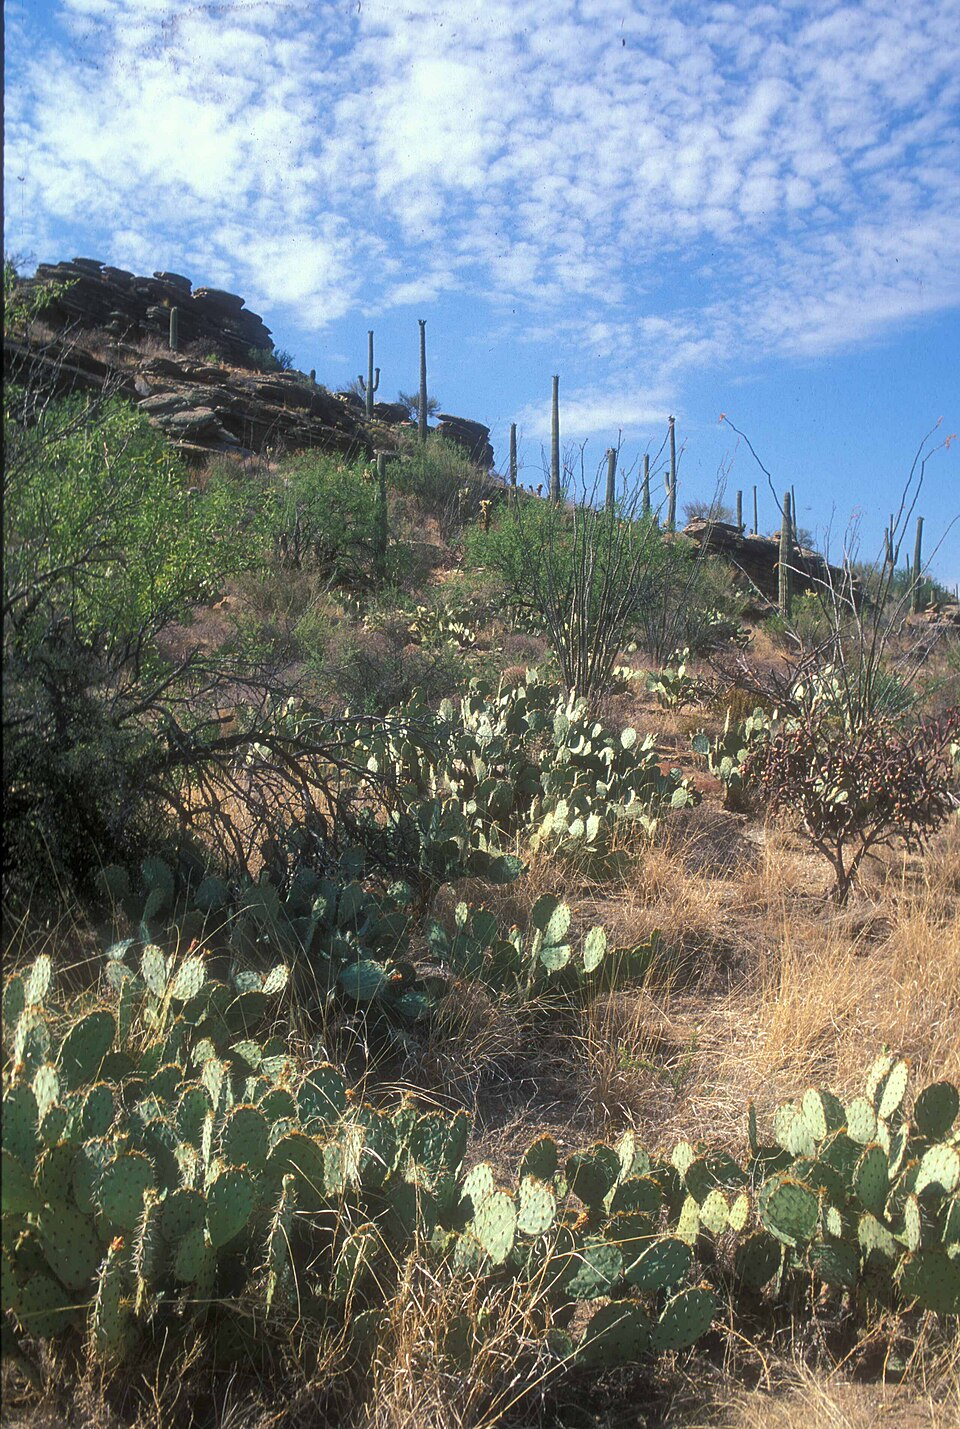
\includegraphics[height=3.6cm]{images/book1/g5-sonoran-desert.jpg}\quad
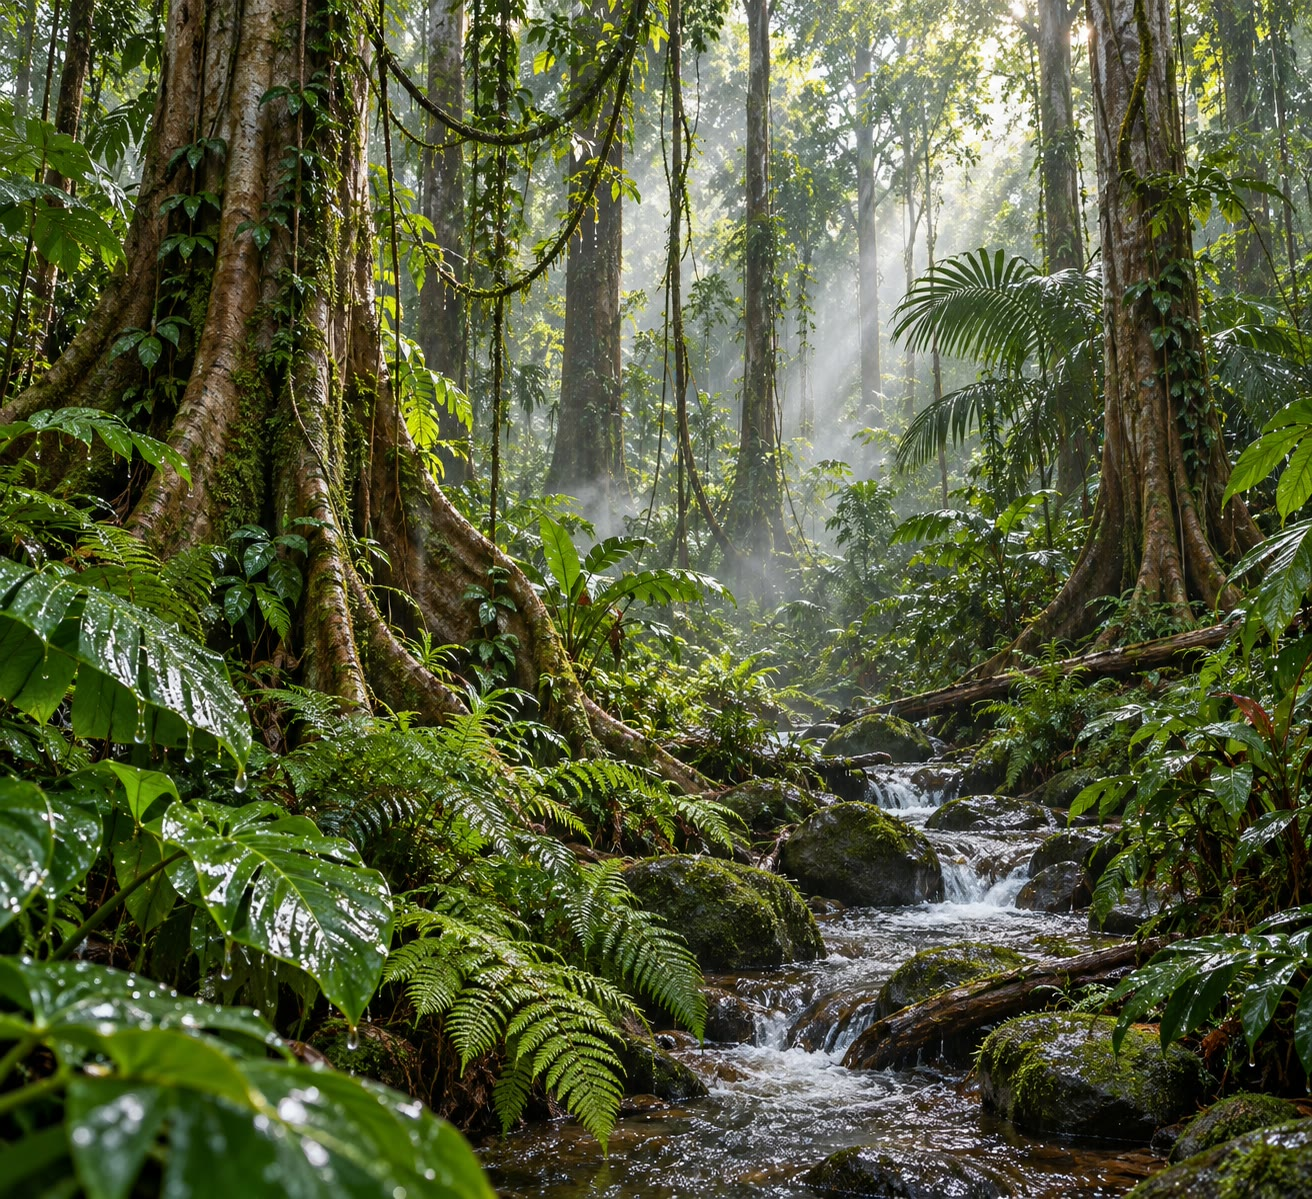
\includegraphics[height=3.6cm]{images/book1/ai/g5-rainforest.jpg}\quad
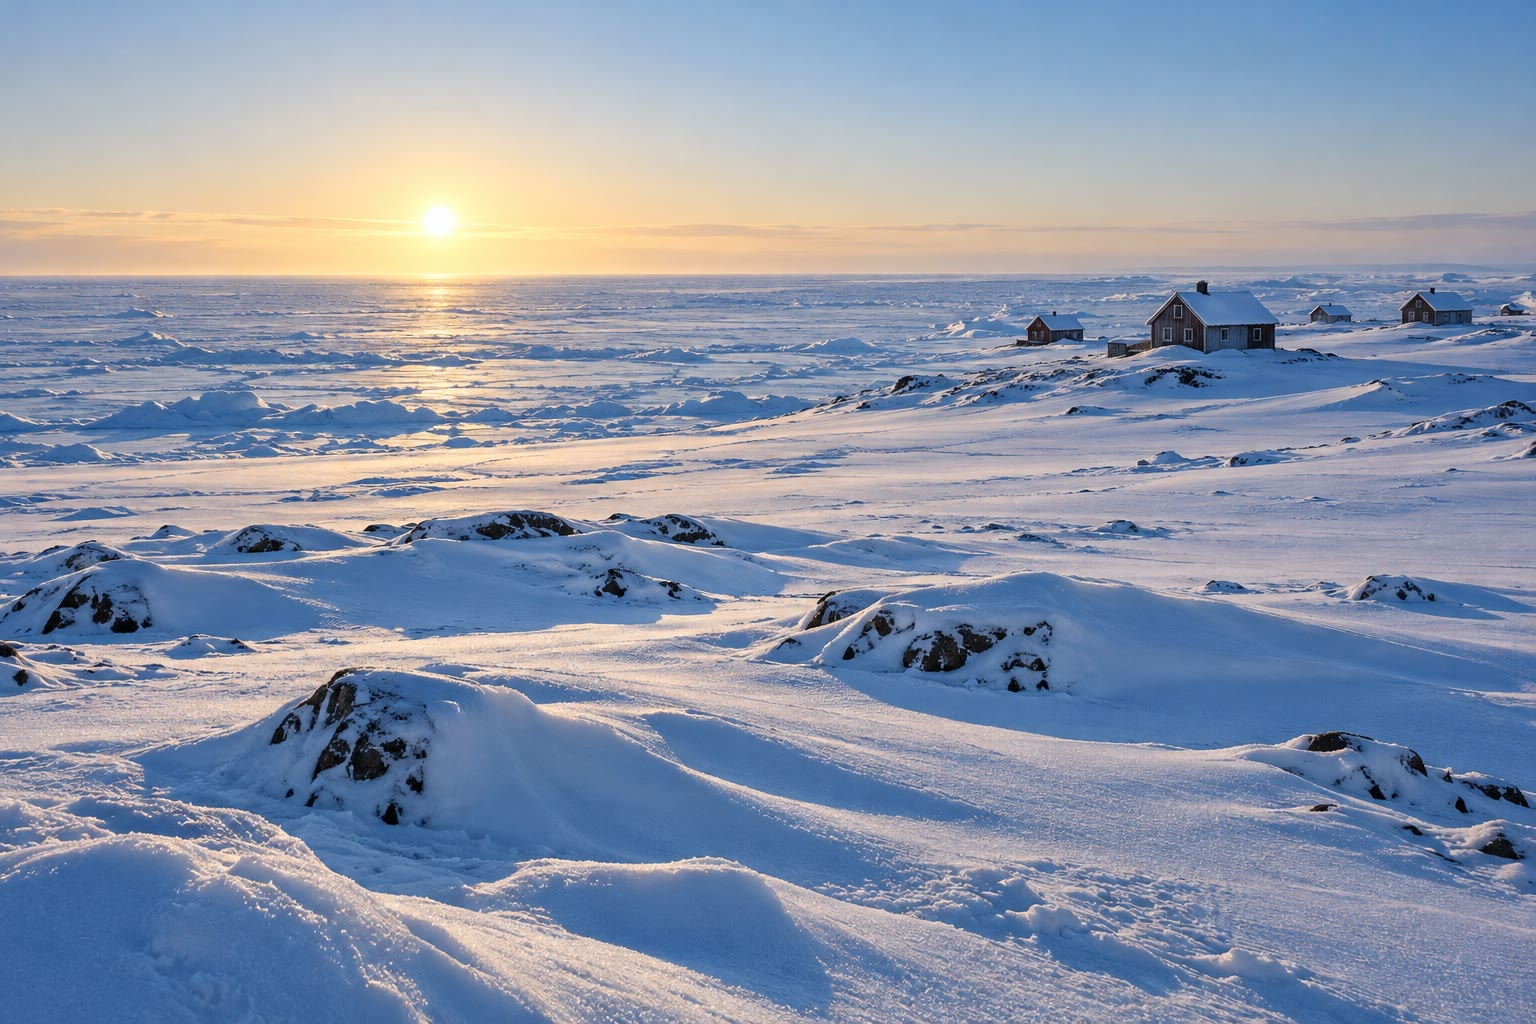
\includegraphics[height=3.6cm]{images/book1/ai/g5-polar-tundra.jpg}

{\small तीन चरम \omterm{def:g5:weather-and-climate:climate}{जलवायु}। बाएँ: एरिज़ोना का सोनोरन \omterm{def:g5:weather-and-climate:desert}{मरुस्थल}, फ़ीनिक्स का \omterm{def:g5:weather-and-climate:desert}{मरुस्थल},
ऊँचे सगुआरो कैक्टस और नागफनी के साथ, जो अपने मोटे तनों में पानी जमा करते हैं
(चित्र: अमेरिकी राष्ट्रीय उद्यान सेवा, सगुआरो राष्ट्रीय उद्यान, सार्वजनिक
डोमेन)। बीच में: बौछार के बाद एक \omterm{def:g5:weather-and-climate:rainforest}{वर्षावन} के अंदर।
दाएँ: सर्दी में एक ध्रुवीय \omterm{def:g1:landscapes-around-us:water}{तट}, जमे हुए \omterm{def:g2:water-on-earth:ocean}{समुद्र} और दोपहर के नीचे सूर्य के साथ।}
% ledger: nps:sonoran-desert
\end{omfigure}

\paragraph{शीतोष्ण जलवायु।} सिएटल बीच में है: उसका वक्र गर्मी में चढ़ता है और सर्दी
में उतरता है, पर कभी बहुत दूर नहीं; वहाँ ठीक-ठाक \omterm{def:g4:clouds-rain-snow:precipitation}{बारिश} होती है, ज़्यादातर पतझड़
और सर्दी में। यह शीतोष्ण \omterm{def:g5:weather-and-climate:climate}{जलवायु} है: न बहुत गर्मी,
न बहुत ठंड।

\paragraph{ध्रुवीय जलवायु।} उत्कियाग्विक में लाल वक्र साल के आठ महीने
0~$^\circ$C से नीचे रहता है; फ़रवरी में औसत शून्य से
24 डिग्री नीचे है। जुलाई में भी, जो सबसे गरम महीना है, वह केवल लगभग
5 डिग्री होता है।
% ledger: data:b1-noaa-normals

\section{उष्ण, शीतोष्ण और शीत कटिबंध}

\omterm{def:g3:continents-and-oceans:equator}{भूमध्य रेखा} के पास गरमी और \omterm{def:g3:continents-and-oceans:poles}{ध्रुवों} के पास ठंड क्यों है? सूर्य के कारण। \omterm{def:g3:continents-and-oceans:equator}{भूमध्य रेखा}
के पास दोपहर का सूर्य पूरे साल आसमान में ऊँचा रहता है: उसकी रोशनी लगभग सीधी नीचे
पड़ती है और ज़मीन को ख़ूब गरम करती है। \omterm{def:g3:continents-and-oceans:poles}{ध्रुवों} के पास सूर्य हमेशा नीचा रहता है:
उसकी रोशनी तिरछी आती है, एक बड़े क्षेत्र पर फैलकर, और कम गरम करती है। वहाँ
सर्दी में सूर्य शायद
उगे ही नहीं।

\omterm{def:g3:continents-and-oceans:globe}{ग्लोब} के चारों ओर की रेखाओं के दो जोड़े पृथ्वी को \omterm{def:g5:weather-and-climate:climate-zone}{जलवायु कटिबंधों} में बाँटते हैं।

\begin{definition}[अयन वृत्त और ध्रुवीय वृत्त]\label{def:g5:weather-and-climate:tropics}
दोनों \emph{अयन वृत्त}\index{अयन वृत्त} \omterm{def:g3:continents-and-oceans:globe}{ग्लोब} के चारों ओर की वे रेखाएँ हैं, एक
\omterm{def:g3:continents-and-oceans:equator}{भूमध्य रेखा} के उत्तर में और एक दक्षिण में, जो दिखाती हैं कि \omterm{def:g3:continents-and-oceans:equator}{भूमध्य रेखा} से कितनी
दूर तक दोपहर का सूर्य ठीक सिर के ऊपर आ सकता है: उत्तर में कर्क रेखा, दक्षिण में
मकर रेखा। दोनों \emph{ध्रुवीय
वृत्त}\index{ध्रुवीय वृत्त} \omterm{def:g3:continents-and-oceans:poles}{ध्रुवों} के पास \omterm{def:g3:continents-and-oceans:globe}{ग्लोब} के चारों ओर की वे रेखाएँ हैं,
जिनके आगे सर्दी के बीच में कम से कम एक दिन सूर्य नहीं उगता, और गर्मी के बीच में
वह नहीं डूबता: उत्तर में आर्कटिक
वृत्त, दक्षिण में अंटार्कटिक वृत्त।
\end{definition}

पृथ्वी के अक्ष का झुकाव तय करता है कि ये रेखाएँ कहाँ हैं।

\begin{definition}[जलवायु कटिबंध]\label{def:g5:weather-and-climate:climate-zone}
पृथ्वी तीन तरह के \emph{जलवायु कटिबंधों}\index{जलवायु कटिबंध} में बँटी है: \emph{उष्ण कटिबंध}, दोनों \omterm{def:g5:weather-and-climate:tropics}{अयन वृत्तों} के बीच, \omterm{def:g3:continents-and-oceans:equator}{भूमध्य रेखा} के चारों ओर;
दो \emph{शीतोष्ण कटिबंध}, एक \omterm{def:g5:weather-and-climate:tropics}{अयन वृत्त} और एक \omterm{def:g5:weather-and-climate:tropics}{ध्रुवीय वृत्त} के बीच, जहाँ
गर्मियाँ और सर्दियाँ अलग होती हैं; और दो \emph{शीत कटिबंध}, \omterm{def:g5:weather-and-climate:tropics}{ध्रुवीय वृत्तों} के
आगे, \omterm{def:g3:continents-and-oceans:poles}{ध्रुवों} के चारों ओर।
\end{definition}

\begin{omfigure}
\begin{tikzpicture}
\begin{axis}[ommap, width=\linewidth, xtick=\empty, ytick=\empty, grid=none,
    axis background/.style={fill=white}, clip=true]
  \addplot[fill=orange!35, draw=none] table {figdata/out/grade-5-climate_zones-hot.dat};
  \addplot[fill=green!20, draw=none] table {figdata/out/grade-5-climate_zones-temperate.dat};
  \addplot[fill=cyan!20, draw=none] table {figdata/out/grade-5-climate_zones-cold.dat};
  \addplot[fill=black!25, fill opacity=0.8, draw=black!60, line width=0.2pt]
    table {figdata/out/shared-geo-land.dat};
  \addplot[black!70, dashed, line width=0.5pt] table {figdata/out/grade-5-climate_zones-lines.dat};
  \draw[black!70, line width=0.6pt] (axis cs:-180,0) -- (axis cs:180,0);
  \addplot[only marks, mark=*, mark size=1.8pt, red!80!black]
    table[x=lon, y=lat] {figdata/out/grade-5-climate_zones-stations.dat};
  \begin{scope}[every node/.style={font=\scriptsize, fill=white, fill opacity=0.75,
      text opacity=1, inner sep=1pt}]
    \node[anchor=west] at (axis cs:-107,33.4) {फ़ीनिक्स};
    \node[anchor=east] at (axis cs:-158,19.7) {हिलो};
    \node[anchor=west] at (axis cs:-117,47.4) {सिएटल};
    \node[anchor=west] at (axis cs:-151,73.5) {उत्कियाग्विक};
  \end{scope}
  \begin{scope}[every node/.style={font=\scriptsize\bfseries, align=center,
      fill=white, fill opacity=0.7, text opacity=1, inner sep=1pt}]
    \node at (axis cs:-5,83) {शीत कटिबंध};
    \node at (axis cs:-40,40) {शीतोष्ण कटिबंध};
    \node at (axis cs:-25,-8) {उष्ण कटिबंध};
    \node at (axis cs:95,-45) {शीतोष्ण कटिबंध};
    \node at (axis cs:-60,-80) {शीत कटिबंध};
  \end{scope}
\end{axis}
\end{tikzpicture}

{\small \omterm{def:g5:weather-and-climate:climate-zone}{जलवायु कटिबंध}। ऊपर से नीचे, धराशायी रेखाएँ आर्कटिक वृत्त, \omterm{def:g5:weather-and-climate:tropics}{कर्क रेखा}, \omterm{def:g5:weather-and-climate:tropics}{मकर
रेखा} और अंटार्कटिक वृत्त हैं; अखंड रेखा \omterm{def:g3:continents-and-oceans:equator}{भूमध्य रेखा} है। लाल बिंदु ऊपर के \omterm{def:g5:weather-and-climate:climate-chart}{जलवायु
आलेखों} वाले चार
शहर हैं।}
% ledger: earth:obliquity, data:b1-noaa-normals
\end{omfigure}

कटिबंध एक पहली, मोटी तस्वीर देते हैं। हर एक के भीतर बहुत-सी दूसरी चीज़ें \omterm{def:g5:weather-and-climate:climate}{जलवायु}
बदलती हैं: कोई जगह \omterm{def:g2:water-on-earth:ocean}{समुद्र} से कितनी दूर है, कितनी ऊँची है, उसकी हवाएँ कहाँ से आती
हैं। तुम उनसे आगे की कक्षाओं में मिलोगे।

\begin{remark}[फ़ीनिक्स और कटिबंध]\label{rem:g5:weather-and-climate:phoenix}
कटिबंधों के \omterm{def:g2:drawing-to-map:map}{मानचित्र} पर फ़ीनिक्स \omterm{def:g5:weather-and-climate:tropics}{कर्क रेखा} से थोड़ा उत्तर में, शीतोष्ण कटिबंध में
है, और फिर भी वह एक गरम \omterm{def:g5:weather-and-climate:desert}{मरुस्थल} है। कटिबंध एक पहली, मोटी तस्वीर हैं: बहुत-से
बड़े गरम \omterm{def:g5:weather-and-climate:desert}{मरुस्थल} \omterm{def:g5:weather-and-climate:tropics}{अयन वृत्तों} के पास, उष्ण कटिबंध के किनारे पर हैं, और इसका कारण
तुम \cref{ch:g8:winds-global-circulation} में
सीखोगे।
\end{remark}

\section{अभ्यास}

\begin{exercise}[$\star$]\label{exo:g5:weather-and-climate:1}
\omterm{def:g1:watching-the-weather:weather}{मौसम} या \omterm{def:g5:weather-and-climate:climate}{जलवायु}?
\begin{enumerate}
  \item[(क)] आज सुबह उत्कियाग्विक में \omterm{def:g4:clouds-rain-snow:precipitation}{हिम} गिर रहा है।
  \item[(ख)] फ़ीनिक्स में गर्मियाँ बहुत गरम और सूखी होती हैं।
  \item[(ग)] कल दोपहर बाद सिएटल में तेज़ हवा चली।
  \item[(घ)] हिलो में साल के हर महीने बहुत \omterm{def:g4:clouds-rain-snow:precipitation}{बारिश} होती है।
\end{enumerate}
\end{exercise}

\begin{exercise}[$\star$]\label{exo:g5:weather-and-climate:2}
किसी जगह की \omterm{def:g5:weather-and-climate:climate}{जलवायु} क्या है? उसका वर्णन करने के लिए मौसम वैज्ञानिक कितने वर्षों के
मापों का औसत निकालते हैं?
\end{exercise}

\begin{exercise}[$\star$]\label{exo:g5:weather-and-climate:3}
सिएटल के \omterm{def:g5:weather-and-climate:climate-chart}{जलवायु आलेख} पर सबसे ठंडा महीना कौन-सा है? सबसे गीला महीना कौन-सा है? क्या
तापमान कभी 0~$^\circ$C से नीचे जाता है?
\end{exercise}

\begin{exercise}[$\star$]\label{exo:g5:weather-and-climate:4}
उत्कियाग्विक के \omterm{def:g5:weather-and-climate:climate-chart}{जलवायु आलेख} पर सबसे गरम महीना कौन-सा है? क्या कोई महीना
10~$^\circ$C से ज़्यादा गरम है?
\end{exercise}

\begin{exercise}[$\star$]\label{exo:g5:weather-and-climate:5}
इनमें से हर जगह किस \omterm{def:g5:weather-and-climate:climate-zone}{जलवायु कटिबंध} में है: \omterm{def:g3:continents-and-oceans:equator}{भूमध्य रेखा}; \omterm{def:g3:continents-and-oceans:poles}{उत्तरी ध्रुव}; \omterm{def:g3:continents-and-oceans:equator}{भूमध्य रेखा}
और \omterm{def:g3:continents-and-oceans:poles}{दक्षिणी ध्रुव} के ठीक आधे रास्ते पर की एक जगह?
\end{exercise}

\begin{exercise}[$\star$]\label{exo:g5:weather-and-climate:6}
कटिबंधों के \omterm{def:g2:drawing-to-map:map}{मानचित्र} का प्रयोग करो। चारों शहरों में से हर एक किस \omterm{def:g5:weather-and-climate:climate-zone}{जलवायु कटिबंध} में
है: फ़ीनिक्स, हिलो, सिएटल, उत्कियाग्विक?
\end{exercise}

\begin{exercise}[$\star\star$]\label{exo:g5:weather-and-climate:7}
यह सिएटल में हर महीने की औसत \omterm{def:g4:clouds-rain-snow:precipitation}{बारिश} है, मिलीमीटर में, पूर्ण संख्याओं में
पूर्णांकित (1 जनवरी है और 12 दिसंबर):
\begin{center}
\begin{tabular}{|*{12}{c|}}
\hline
1 & 2 & 3 & 4 & 5 & 6 & 7 & 8 & 9 & 10 & 11 & 12\\
\hline
147 & 96 & 106 & 81 & 48 & 37 & 15 & 25 & 41 & 99 & 160 & 145\\
\hline
\end{tabular}
\end{center}
सिएटल में पूरे साल में कितनी \omterm{def:g4:clouds-rain-snow:precipitation}{बारिश} गिरती है? दिसंबर, जनवरी और फ़रवरी, इन तीन
महीनों में कितनी गिरती है?
% ledger: data:b1-noaa-normals
\end{exercise}

\begin{exercise}[$\star\star$]\label{exo:g5:weather-and-climate:8}
फ़ीनिक्स में औसत तापमान जनवरी में 14~$^\circ$C और जुलाई में
35~$^\circ$C है। हिलो में वह जनवरी में 22~$^\circ$C और जुलाई में
25~$^\circ$C है। हर शहर में जुलाई और जनवरी का अंतर निकालो। ऋतुएँ तापमान को
कहाँ ज़्यादा बदलती हैं?
% ledger: data:b1-noaa-normals
\end{exercise}

\begin{exercise}[$\star\star$]\label{exo:g5:weather-and-climate:9}
यह एक काल्पनिक शहर के औसत हैं।
\begin{center}
\begin{tabular}{|l|*{12}{c|}}
\hline
महीना & 1 & 2 & 3 & 4 & 5 & 6 & 7 & 8 & 9 & 10 & 11 & 12\\
\hline
तापमान ($^\circ$C) & 27 & 27 & 28 & 28 & 28 & 27 & 27 & 27 & 27 & 27 & 27 & 27\\
\hline
\omterm{def:g4:clouds-rain-snow:precipitation}{बारिश} (मिमी) & 250 & 230 & 280 & 290 & 260 & 180 & 170 & 160 & 190 & 230 & 250 & 260\\
\hline
\end{tabular}
\end{center}
यह \omterm{def:g5:weather-and-climate:desert}{मरुस्थल}, \omterm{def:g5:weather-and-climate:rainforest}{वर्षावन}, शीतोष्ण या ध्रुवीय, किस तरह की \omterm{def:g5:weather-and-climate:climate}{जलवायु} है? दो कारण बताओ।
यह शहर सबसे ज़्यादा संभावना से किस कटिबंध में होगा?
\end{exercise}

\begin{exercise}[$\star\star$]\label{exo:g5:weather-and-climate:10}
अध्याय की शुरुआत के उन दो पोस्टकार्डों पर लौटो, जो जनवरी के एक ही हफ़्ते में भेजे
गए थे। इसकी दो अलग-अलग व्याख्याएँ दो कि कैसे एक जगह बच्चे धूप वाले \omterm{def:g2:water-on-earth:ocean}{समुद्र} \omterm{def:g1:landscapes-around-us:water}{तट} पर
खेल सकते हैं जबकि दूसरी जगह दूसरे बच्चे हिम-पुतला बनाते हैं।
\end{exercise}

\begin{exercise}[$\star\star\star$]\label{exo:g5:weather-and-climate:11}
नूर कहती है: ``फ़ीनिक्स और सिएटल दोनों शीतोष्ण कटिबंध में हैं, इसलिए उनकी \omterm{def:g5:weather-and-climate:climate}{जलवायु}
एक-सी ही होनी चाहिए।'' \omterm{def:g5:weather-and-climate:climate-chart}{जलवायु आलेखों} से दिखाओ कि वह ग़लत है: उनके तापमानों और
उनकी \omterm{def:g4:clouds-rain-snow:precipitation}{बारिश} की तुलना करो। फिर बताओ कि \omterm{def:g5:weather-and-climate:climate-zone}{जलवायु कटिबंध} हमें क्या बताते हैं, और क्या
नहीं बताते।
\end{exercise}
